% This section covers the content of 'Social Science Research:
% Principles, Methods, and Practices (2012) by Anol Bhattacherjee',
% Chapters 1-4, 5, 6 and 13.
% I also interspersed some content from Todd Landman's book on Comparative
% Politics.
\section{Social Science Research: Principles, Methods, and Practices}

% SSR chapter 1
% Block 1
\subsection{Science and Scientific Research}
\begin{flushright}
  \scriptsize Notes from `Social Science Research: Principles, Methods, and
  Practices' (2012) by Anol Bhattacherjee, Chapter 1. Block 1.
\end{flushright}

\defn{Science}{Is the systematic and organized body of knowledge in
  any area of inquiry that is acquired using the ``scientific
  method''.}

\defn{Natural Sciences}{Are the sciences of naturally occurring objects
  or phenomena, such as light, objects, matter, earth, etc. Natural
  Sciences can be further broken down into physical sciences, earth
  sciences, life science, etc.}

\defn{Social Sciences}{Are the sciences of people or collections of
  people (such as groups, firms, economies, societies) and their
  behaviours. These sciences include psychology, sociology and
  economics.}

\defn{(Scientific) Laws}{Are observed patterns of phenomena or
  behaviour.}

\defn{(Scientific) Theories}{Are systematic explanations of the
  underlying phenomenon or behaviour.}

Sometimes, there may not be a `single universal truth', rather there
could be an equilibrium of `multiple truths'. We arrive at scientific
laws and theories through logic (theory) and evidence
(observation). Theories provide meaning and significance to what we
observe, and observations help validate or refine existing theory, or
construct new theories. As such, science operates at two levels; the
\textbf{theoretical level} and the \textbf{empirical level}.

% Inductive:
% Bob is human, Bill is human, Anne is human (cases)
% Bob, Bill and Anne have all died (results)
% Humans are mortal (conclusion/rule)
% Deductive
% Humans are mortal (rule)
% Bob, Bill and Anne are humans (cases)
% Therefore Bob, Bill and Anne are mortal (results)
\marginpar{QQ: Give an example of a inductive and deductive argument.}

\defn{Inductive Research (theory building)}{Involves the researcher
  inferring theoretical concepts and patterns from observed data.}

\defn{Deductive Research (theory testing)}{Involves the researcher
  testing concepts and patterns from a known theory using new
  empirical data.}

\marginpar{You can think of inductive research as `inducing' a theory
  from data.}

\begin{center}
  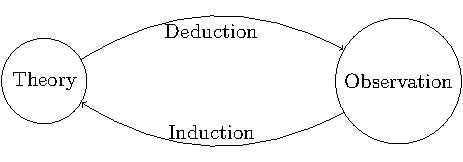
\includegraphics{cycle-of-research.pdf}
\end{center}

Theory building and theory testing are especially hard for social
sciences, since theoretical concepts in the social sciences are
usually imprecise, with inadequate measuring tools and many
unaccounted factors.

\subsubsection{The Scientific Method}

The Scientific Method refers to a standardized set of techniques for
building scientific knowledge. It allows researchers to independently
and impartially test preexisting theories and prior findings and
subject them to open debate, modifications or enhancements.

The scientific method must have four characteristics:

\begin{adjustwidth}{0.5cm}{}
\begin{description}
  \item[Logical] Scientific inferences must be based on logical principles of reasoning.
  \item[Confirmable] Inferences derived must match with observed evidence.
  \item[Repeatable] Other scientists should be able to independently
    replicate or repeat a scientific study to obtain similar or
    identical results.
  \item[Scrutinizable] The procedures used and the inferences derived
    must withstand peer review by other scientists.
\end{description}
\end{adjustwidth}

\subsubsection{Types of Scientific Research}

There are three types of scientific research:

\marginpar{QQ: Try to think of examples of each type of research.}

\begin{description}
  \item[Exploratory research] is usually conducted in new areas of
    inquiry, where the goals are to scope out a phenomenon, generate
    some ideas, or test the feasibility of undertaking a more expensive
    study.
  \item[Descriptive research] is directed at making careful
    observations and detailed documentation of a phenomenon of
    interest. This is the `what', `where' and `when' questions.
  \item[Explanatory research] seeks explanations of observed phenomena,
    problems or behaviours. The `why' and `how' types of questions.
\end{description}

% Note that I've skipped the `history of scientific thought' section
% since I don't think it'll come up on the exam, but I should probably
% learn it anyway since the history and terminology is likely useful.

% SSR chapter 2
% Block 1
\subsection{Thinking Like a Researcher}
\begin{flushright}
  \scriptsize Notes from `Social Science Research: Principles, Methods, and
  Practices' (2012) by Anol Bhattacherjee, Chapter 2. Block 1.
\end{flushright}

Researchers must constantly move back and forth between the
\textit{empirical plane} where observations are conducted and the
\textit{theoretical plane} where the observations are abstracted into
general laws and theories.

\defn{Unit of analysis}{Refers to the person, collective, or object
  that is the target of the investigation.}

You should always measure variables at an appropriate level of
semantic meaning to the unit of analysis. For instance, if your unit
of analysis is an organization (a charity, corporation, NGO, etc),
then the variables you might measure could be the size of the
organization, revenue, hierarchy, employee pay ratio etc.

\defn{Concepts}{Are generalizable properties or characteristics
  associated with objects, events or people.}

\defn{Construct}{A construct is an abstract concept that is
  specifically chosen (or created) to explain a given
  phenomenon. Constructs can be \textbf{unidimensional} such as
  somebody's weight, or \textbf{multidimensional} such as somebody's
  communication skills.}

\defn{Operational definitions}{Are used for scientific research (in
  place of dictionary definitions), and define constructs in terms of
  how they will be empirically measured. For example, the operational
  definition of temperature will explain what unit it will be measured
  in.}

\defn{Variable}{A variable is a measurable representation of an
  abstract construct.}

\begin{figure}[H]
  \begin{center}
    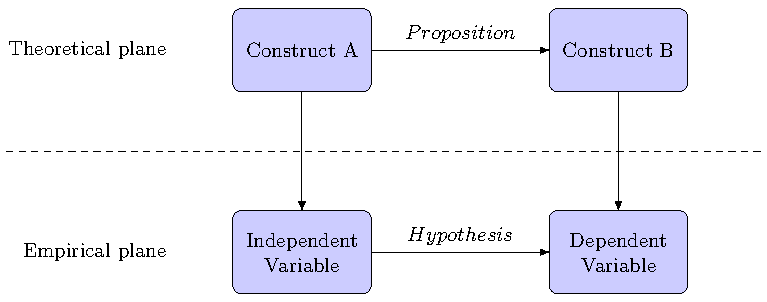
\includegraphics[width=\textwidth]{planes-of-research.pdf}
  \end{center}
  \caption{The theoretical and empirical planes of research.}
\end{figure}

\marginpar{Try to give an example of each type of variable.}

Depending on their use, variables may be classified into different
types:
\begin{description}
  \item \defn{Independent Variables}{Are variables that explain other
    variables.}
  \item \defn{Dependent Variables}{Are variables that are explained by
    other variables.}
  \item \defn{Mediating Variables}{Also known as intermediate variables
    are those that are explained by an independent variable, but also
    explain a dependent variable}
  \item \defn{Moderating Variables}{Influence the relationship between
    independent and dependent variables.}
  \item \defn{Control Variables}{Must be monitored or kept constant during
    a scientific study.}
\end{description}

\begin{figure}[H]
  \begin{center}
    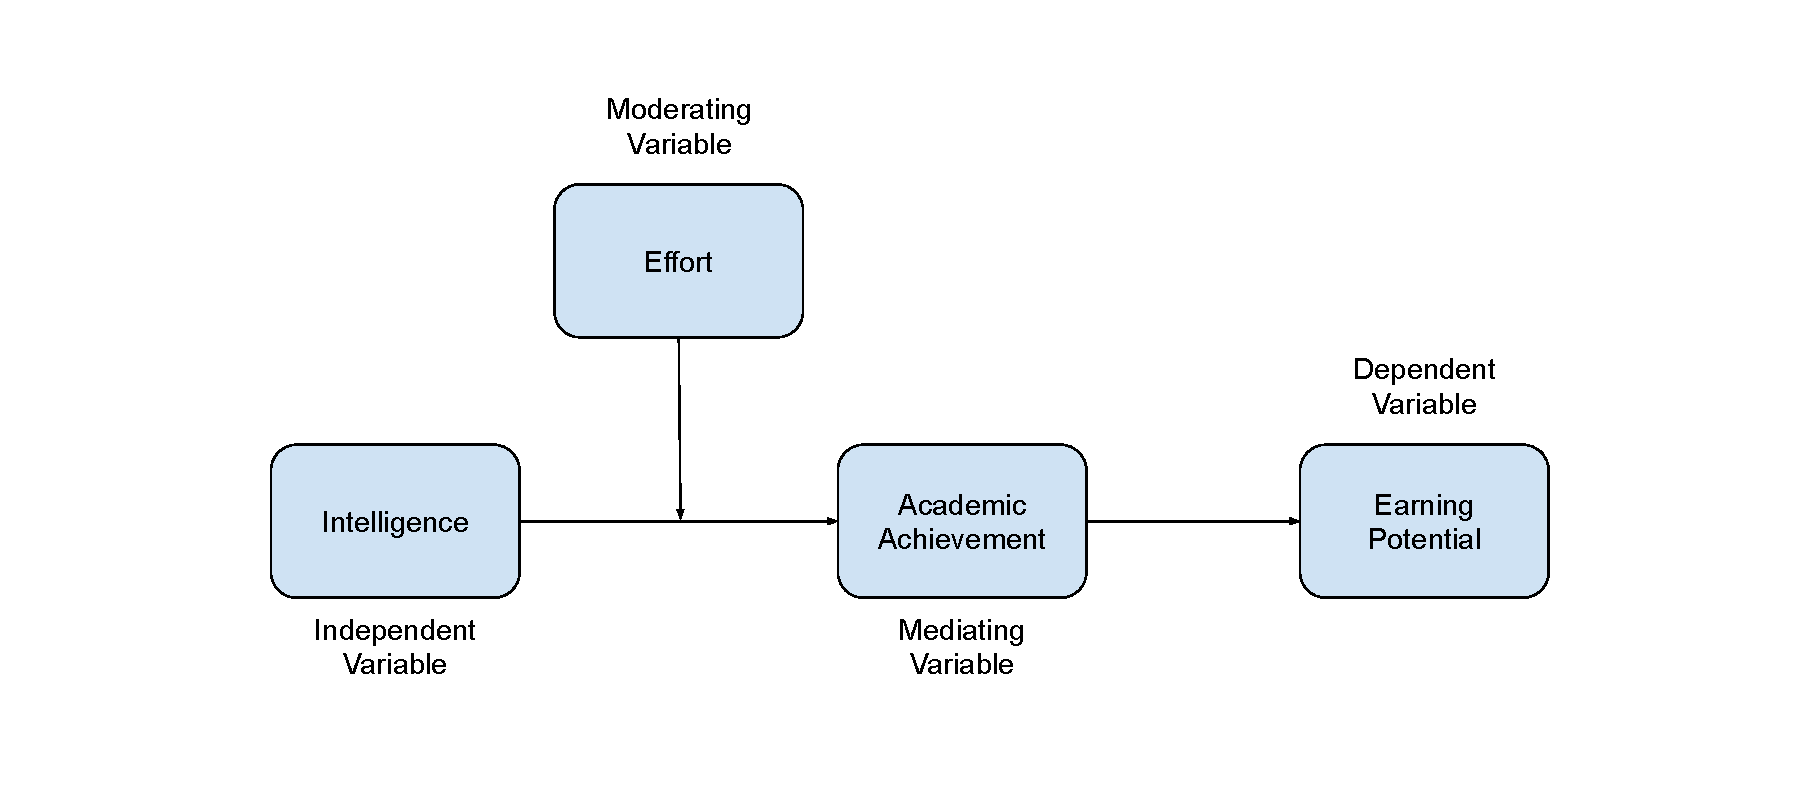
\includegraphics[width=\textwidth]{network-of-constructs.pdf}
  \end{center}
  \caption{An example of different kinds of variables.}
\end{figure}

\defn{Normological Network}{The overall network of relationships
  between a set of related constructs.}

\defn{Proposition}{A tentative and conjectural relationship between
  constructs that is stated in a declarative form. E.g. ``An increase
  in student intelligence causes an increase in their academic
  achievement''. It does not have to be true, but does have to be
  empirically testable using data.}

Propositions (on the theoretical plane) are tested indirectly by
examining the relationships between the variables (on the empirical
plane) that relate to the constructs involved.

\defn{Hypothesis}{A hypothesis is the empirical version of a
  proposition, that is to say that it says something about the
  relationship between variables, with the dependent and independent
  variables clearly specified.}

\defn{Strong Hypothesis}{Is a hypothesis with its directionality and
  causality specified (as opposed to a \textit{weak hypothesis}, which
  specifies neither).}

\defn{Theory}{A theory is a set of systematically interrelated
  constructs and propositions intended to explain and predict a
  phenomenon or behaviour of interest, within certain boundary
  conditions and assumptions.}

A good scientific theory should be well supported using observed
facts, and should also have practical value, while a poorly defined
theory tends to be lacking in these dimensions.

\defn{Model}{A model is a representation of all or part of a system
  that is constructed to study that system. While a theory tries to
  explain a phenomenon, a model tries to represent a phenomenon.}

Models can be descriptive, predictive or normative. Descriptive models
are used for representing complex systems and for visualising
variables and relationships in these systems. Predictive models are
used to forecast future events, and normative models are used to guide
activities along commonly accepted norms or practices.

\begin{figure}[H]
  % Diagram can be found at:
  % https://docs.google.com/document/d/1gQDxyFhq5kGWZhtcXF9zL1LTRiFKuTIL_4DNzE_93qA/edit?usp=sharing
  \begin{center}
    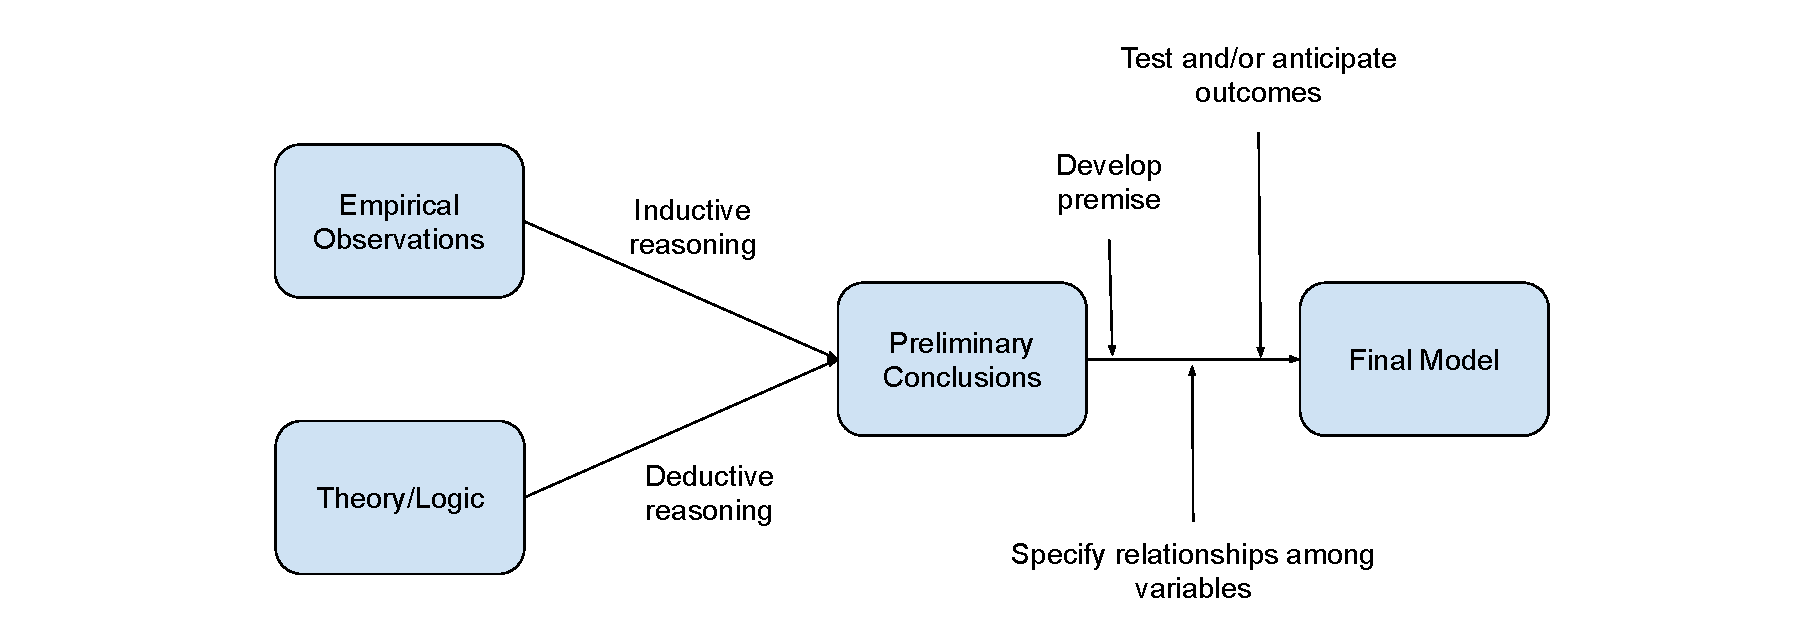
\includegraphics[width=\textwidth]{model-building.pdf}
  \end{center}
  \caption{The steps required to build a model.}
\end{figure}

% SSR chapter 3
% Block 1
\subsection{Doing Research}
\begin{flushright}
  \scriptsize Notes from `Social Science Research: Principles, Methods, and
  Practices' (2012) by Anol Bhattacherjee, Chapter 3. Block 1.
\end{flushright}

\defn{Paradigm}{A paradigm is a mental model or frame of reference
  that we use to organize our reasoning and observations. They are
  often hard to recognize because they are implicit, assumed and taken
  for granted.}

Looking at the same problem through different `lenses' can give
different conclusions. Looking with a rational lens may produce
rational explanations, looking with a social lens may produce
explanations focusing on social deficiencies, and looking through a
political lens may produce political solutions. As such, a `lens' is
like a subconscious paradigm that constrains the concepts that
researchers attempt to use when understanding a phenomenon. Often,
multiple paradigms or lenses will be simultaneously and partially
correct; only by applying several can a researcher gain a full
appreciation of the problem.

\defn{Positivism}{Says that knowledge creation is restructured to what
  can be observed and measured, tending towards theories that can be
  directly tested (and positively confirmed).}

\defn{Post-positivism}{Post-positivism argues that one can make
  reasonable inferences about a phenomenon by combining empirical
  observations with logical reasoning.}

\defn{Ontology}{Refers to our assumptions about how we see the world.}

\defn{Epistemology}{Refers to assumptions about the best way to study
  the world.}

\defn{Methodology}{Concerns the ways in which knowledge of the
  political world is acquired.}

As such, these three concepts have a `directional dependence';
ontology establishes what is knowable, epistemology establishes how it
is knowable, and methodology establishes how the knowledge is
systematically acquired.

\defn{Micro-political analysis}{Examines the political activity of
  individuals such as respondents in a mass survey or politicians.}

\defn{Macro-political analysis}{Focuses on groups of individuals,
  structures of power, social classes, economic processes, and the
  interaction of nation states.}

% There are four paradigms of social science research:
%\begin{description}
%  \item[Functionalism] Studying the social order of the world (patterns
%    of ordered events and behaviours) using an objective approach that
%    is independent of the person studying the pheonomena, and using
%    standard data collection.
%  \item[Interpretivism] Studying the social order of the world from the
%    subjective viewpoint of the people involved, and evaluating their
%    responses using the researcher's own subjective perspectives.
%  \item[Radical structuralism] Believing that the world consists of
%    radical change, and that it should be studied using standardized
%    data collection.
%  \item[Radical humanism] ??? This seems to be the same as number
%    interpretivism according to the description.
%\end{description}

\subsubsection{The research process}

Research is an iterative process, characterized by
\textbf{observation} where phenomena are observed,
\textbf{rationalization} which tries to make sense of these phenomena,
and then \textbf{validation} which tries to confirm that the outcome
of the rationalization stage correctly confirms the phenomena from the
observation stage.

Functionalist research has three stages, \textbf{exploration},
\textbf{research design}, and \textbf{research execution}.

The \textbf{exploration} stage consists of three components:
\begin{adjustwidth}{0.5cm}{}
\begin{description}
  \item[Research questions] Figuring out specific questions you want to
    answer
  \item[Literature review] Surveying the current state of knowledge,
    identifying key authors, theories and articles, and identifying
    gaps in knowledge.
  \item[Theory] Finding a theory to help answer the research questions
    (which helps figure out how constructs are interrelated to the
    target phenomenon).
\end{description}
\end{adjustwidth}

\textbf{Research design} is concerned with figuring out \textit{how}
the research will be carried out. It has three components:
\begin{adjustwidth}{0.5cm}{}
\begin{description}
  \item[Operationalization] The process of designing precise measures
    for abstract theoretical constructs, including specifying
    `operational definitions' for each construct in the theory in the
    context of the observed phenomena.
  \item[Research method] What method will be used for collecting data;
    including quantitative (experiments or surveys) and qualitative
    methods (e.g. case studies).
  \item[Sampling strategy] which is a method to select individual
    entities from a population to study.
\end{description}
\end{adjustwidth}

Once the research is designed, a \textbf{research proposal} will be
written, explaining the decisions made so far, and their rationale.

\marginpar{QQ: Draw a diagram of the research process.}

Once the research proposal is accepted, the research execution phase
begins. This includes:
\begin{adjustwidth}{0.5cm}{}
\begin{description}
  \item[Pilot testing] which helps detect potential problems in the
    research design or instrumentation.
  \item[Data collection] from the sampled population.
  \item[Data analysis] which includes interpreting the data and
    drawing conclusions about it.
  \item[Research report] which could be a dissertation, paper, etc. It
    should details the whole process, from the start to the analysis
    of the results and the conclusion.
\end{description}
\end{adjustwidth}

\subsubsection{Common research mistakes}

\begin{description}
  \item[Insufficiently motivated research questions] The research
    question must be related to a real problem that affects real people.
  \item[Pursuing research fads] Popular topics often have a limited
    shelf life, and by the time the paper is published, the topic
    might have become boring again. Timeless topics are better
    research areas.
  \item[Unresearchable problems] These include problems without much
    evidence, ambiguously defined problems, or problems that cannot be
    solved with currently accepted methods and procedures.
  \item[Favoured research methods] Research methods should be chosen
    to best fit a research problem, and not the other way around.
  \item[Blind data mining] The researcher should not collect the data
    first, and try to fit a theory to it later. The data collection
    must be directed by the planning stages of the research, and an
    abundance of data cannot make for deficits in the research
    planning stage.
\end{description}

% SSR chapter 4
% Block 1
\subsection{Theories in Scientific Research}
\begin{flushright}
  \scriptsize Notes from `Social Science Research: Principles, Methods, and
  Practices' (2012) by Anol Bhattacherjee, Chapter 4. Block 1.
\end{flushright}

\defn{Idiographic explanations}{Are those that explain a single
  situation or event in idiosyncratic detail, e.g.  if you failed an
  exam because you forgot it, because you arrived late, you panicked,
  or had a hangover. They are not generalizable.}

\defn{Nomothetic explanations}{Are explanations that seek to explain
  a class of situations or events rather than a specific situation or
  event. E.g. generally, students can fail exams because they don't
  spend enough time studying. They are less precise and less complete
  than idiographic explanations, but are also economical in their
  explanations and use few variables. Theories are usually
  nomothetic.}

Theories are useful, since they provide the underlying logic of what's
happening by explaining key drivers and outcomes, and why they
occur. They also help synthesize prior empirical findings into a
framework, reconcile contradictory findings, provide guidance for
future research, and bridge gaps between other theories to connect
different areas of research.

\subsubsection{Building a Theory}

\marginpar{QQ: What are the four building blocks of a theory? Don't
  look!}

There are four building blocks of a theory:
\begin{description}
  \item[Constructs] which capture the ``what''. They are abstract
    concepts that are chosen specifically to explain the phenomenon of
    interest. They must have a clear operational definition, and their
    real-world forms on the empirical plane  are variables.
  \item[Propositions] which capture the ``how'', are associations
    between constructs based on deductive logic, and stated in
    declarative form (i.e. if $X$ happens, then $Y$ follows). They
    must be testable, and their real-world forms on the empirical plane
    are hypotheses.
  \item[Logic] which is the ``why'', provides a basis for justifying
    the propositions, and explain the core of the theory.
  \item[Boundary conditions or assumptions] which are the ``who'',
    ``when'', ``where'', etc (i.e. all the circumstances that the
    reified instances of the theory occur in). The boundary conditions
    say when and where the theory can be applied to practice.
\end{description}

\subsubsection{Attributes of a Good Theory}

A good theory has the following attributes:

\begin{itemize}
  \item It is logically consistent, and all its parts fit together in a
    reasonable way.
  \item It can explain or predict reality well, or at least better
    than rival theories.
  \item It must be falsifiable, ensuring that it's possible to find
    data that contradicts the theory, in which case the theory would
    be disproven.
  \item Good theories are parsimonious, and explain a phenomenon with
    few variables.
\end{itemize}

\defn{Occam's razor}{States that among competing explanations that
  sufficiently explain the observed evidence, the most simple theory
  is usually the best.}

\subsubsection{Approaches to Theorizing}

\defn{Grounded theory building}{Is building theories based on observed
  patterns of events or behaviours. The theory is `grounded' in
  empirical observations. The researcher must provide a consistent
  explanation for all the patterns.}

A \textbf{bottom-up conceptual analysis} can identify different sets
of predictors relevant to a phenomenon by examining different
inputs/variables, and describing the underlying processes that link
them to the target phenomenon.

Another approach, can be to extend or modify existing theories to
explain a new situation. This can be very efficient. Or, existing
theories can be applied in an entirely new context, by drawing
similarities between the original context of the theory and the new
context where it is applied.

% SSR chapter 5
% Block 2
\subsection{Research Design}
\begin{flushright}
  \scriptsize Notes from `Social Science Research: Principles, Methods, and
  Practices' (2012) by Anol Bhattacherjee, Chapter 5. Block 2.
\end{flushright}


\defn{Internal Validity}{Examines whether the observed change in a
  dependent variable is indeed caused by a corresponding change in the
  independent variable, and not by other variables. Internal validity
  requires that the effect happens if the cause happens (covariation),
  the cause must precede the effect (temporal precedence) and that
  there is no plausible alternative explanation.}

\defn{External Validity}{Refers to whether the observed associations
  can be generalized from the sample to the population.}

\defn{Construct Validity}{Examines how well a given measurement scale
  is measuring the theoretical construct that it is expected to
  measure. E.g. if empathy is being measured, it must be asserted that
  it's not actually compassion being measured.}

\defn{Statistical Conclusion Validity}{Examines the extend that
  conclusions derived using a statistical procedure are valid.}

\begin{figure}[H]
  \begin{center}
    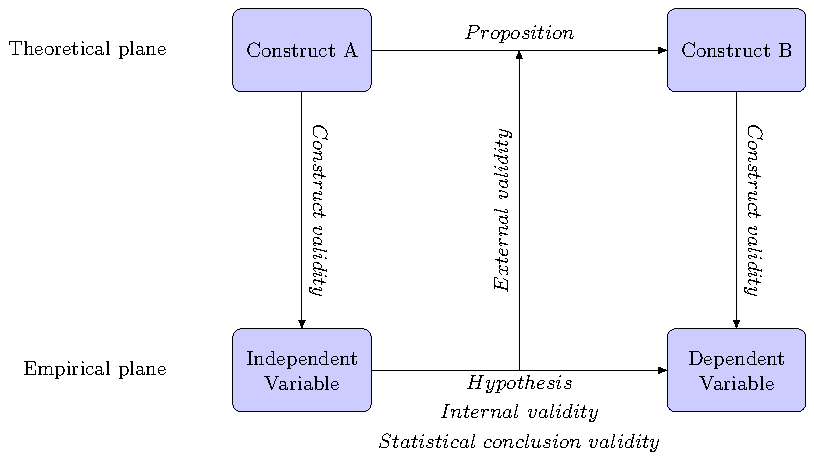
\includegraphics[width=\textwidth]{planes-of-research-2.pdf}
  \end{center}
  \caption{The theoretical and empirical planes of research, annotated
    with the different types of validity.}
\end{figure}

In order to improve validity, the following controls can be
implemented:

\begin{description}
  \item[Manipulation] The researcher manipulates the independent
    variables and compares the effects against a control group.
  \item[Elimination] Tries to eliminate extraneous variables by making
    them constant, e.g. by restricting a study to a single gender.
  \item[Inclusion] Is when the researcher tries to account for the
    effect of extraneous variables by estimating their effects on the
    dependent variable, then accounting for the effect in the results.
    \marginpar{Randomization assures both internal validity and
      external validity, since inferences drawn from a random sample
      of a population can be generalized to the whole population.}
  \item[Randomization] Is when random sampling is used to cancel out
    the effects of extraneous variables. This can take the form of
    random selection (choosing a sample at random), or random
    assignment (selecting a sample, but randomly assigning them to the
    experiment or control groups).
\end{description}

\subsubsection{Different Research Designs}

\begin{description}
  \item[Experimental studies] Are studies intended to test cause-effect
    relationships in a tightly controlled setting, using an experiment
    group and a control group.
  \item[Field surveys] Do not control for independent variables, but
    measure them and test their effects using statistical
    methods. Cross-sectional field surveys measure the independent and
    dependent variables at the same time, while longitudinal field
    surveys measure the dependent variable after the independent
    variable.
  \item[Secondary data analysis] Is analysis of data previously
    collected by other sources.
  \item[Case research] Is an in-depth investigation of a problem in
    one or more real-life settings.
  \item[Focus group research] Involves bringing a small group of
    subjects into a discussion where they talk about a phenomenon of
    interest.
  \item[Action research] Assumes that complex phenomena are best
    understood by introducing interventions (actions) into them, and
    observing the effects of the interventions.
\end{description}

% SSR chapter 6
% Block 2
\subsection{Measurement of Constructs}
\begin{flushright}
  \scriptsize Notes from `Social Science Research: Principles, Methods, and
  Practices' (2012) by Anol Bhattacherjee, Chapter 6. Block 2.
\end{flushright}

\defn{Conceptualization}{Is the process by which fuzzy and imprecise
  constructs (concepts) are defined in concrete and precise terms.}

Conceptualization is important in social science, since concepts are
often vague or ambiguous. Sometimes, concepts are treated as real, in
which case they are said to be `reified'.

\defn{Operationalization}{Refers to the process of developing
  indicators or items for measuring a construct, which are called
  variables.} These variables operate at the empirical level, while
their corresponding constructs exist on the theoretical level.

Indicators can be \textit{reflective}, meaning that they reflect a
measure of the underlying construct, or \textit{formative}, which
means that they contribute to the definition of the underlying
construct.

\subsubsection{Rating scales}

\defn{Rating scales}{Refer to the values that an indicator can take
  (kind of like the \textit{type} of a variable in a programming
  language.}

\begin{description}
  \item[Nominal scales] Measure categorical data (e.g. gender or
    religion).
  \item[Ordinal scales] Measure values that can be ordered
    (e.g. first, second, third), but the actual values cannot be
    assessed.
  \item[Interval scales] These scales are rank ordered, but are also
    bucketed.
  \item[Ratio scales] Have all the qualities of the above scales, but
    additionally with a `true zero' point.
  \item[Binary scales] Are yes/no values.
  \item[Likert scale] Measures ordinal data, and consists of a
    statement and an extend of a respondent's agreement with the
    statement from 1-5 or 1-7.
  \item[Guttman scale] Uses a series of yes/no questions arranged in
    increasing order of intensity, (e.g. do you think Government
    should be involved in healthcare, do you think Government should
    have financial programmes to fund healthcare, etc).
\end{description}

% I'm skipping `scaling' from Chapter 6 of SSR because I don't think
% it's likely to come up on the exam.

% SSR chapter 13
\subsection{Qualitative Analysis}
\begin{flushright}
  \scriptsize Notes from `Social Science Research: Principles, Methods, and
  Practices' (2012) by Anol Bhattacherjee, Chapter 13. Block 2.
\end{flushright}


Qualitative Analysis is the analysis of qualitative data such as
text data from interview transcripts. The emphasis is in making sense
of a phenomenon, rather than predicting or explaining it.

\marginpar{QQ: What are the qualitative analysis methods?}

\subsubsection{Grounded theory}

\defn{Grounded theory}{Is an inductive technique of interpreting
  recorded data about a social phenomena to build theories about
  it. The interpretations are `grounded in' the observed empirical
  data.}

Grounded theory works in stages:
\begin{enumerate}
  \item \defn{Open coding}{Involves the researcher examining raw textual
    data line-by-line, and identifying discrete events, incidents,
    ideas, actions, perceptions, etc that are coded as concepts. Each
    concept is linked to a specific portion of the text for later
    validation. The technique is called `open' because the researcher
    is open to finding new concepts in the text.}
  \item Concepts are grouped into higher-order categories that are more
    broad and generalizable than the concepts from open coding. Each
    category has characteristics and dimensions that help fit new
    concepts from the open coding into it.
  \item These categories are then grouped in a process called
    \textit{axial coding}, which should start to show their causal
    relationships so a tentative hypothesis can be formed.
  \item Finally, \textit{selective coding} is used to identify a
    central category, and relate that to the other categories.
\end{enumerate}

This process is repeated (with new data being added, and new concepts
being created) until \textit{theoretical saturation} is reached and
new data doesn't yield new concepts.

\subsubsection{Content Analysis}

\defn{Content Analysis}{Is the systematic analysis of the context of a
text (e.g. who says what to whom, why, what are the effects, etc).}

The process is like this:
\begin{enumerate}
\item The researcher chooses a sample set of texts for analysis.
\item The researcher splits each text into chunks which can be treated
  as separate units of analysis. This is called unitizing.
\item The researcher then constructs and applies one or more concepts
  to the unitized text, which is called \textit{coding}.
\item The coded data is analysed to find the themes which occur most
  frequently.
\end{enumerate}

One example of content analysis is \textit{sentiment analysis}, which
analyses a text to capture the opinion or attitude of the writer.

\subsubsection{Hermeneutic Analysis}

\defn{Hermeneutic analysis}{ A special type of content analysis, where
  the researcher tries to ``interpret'' the subjective meaning of a
  given text within its socio-historical context.} The word
\textit{hermeneutic} referees to one particular strand or
interpretation, so hermeneutic\textit{s} refers to them in the
collective.

% The lecture titled 'methods of comparison' from block 1.
\subsection{Methods of Comparison}
\begin{flushright}
  \scriptsize Notes from the lecture titled `Methods of Comparison'
  from Block 1.
\end{flushright}

\marginpar{QQ: What are the three `methods of comparison' designs
  covered here?}

\subsubsection{Most Similar System Design}

`Most similar system design' is a method of comparison defined by
Prezorwski and Teune, and is used to explain differences in outcome
between similar two cases. It looks for an independent variable that
differs between the two cases.

For example, given the question ``Although Sweeden and the US are both
rich democracies, how come crime rates are lower in Sweeden?'', the
most similar system design school might say that it's because the
population is much more homogeneous in Sweeden.

For example, France had a revolution and England did not have a
revolution. They both had expensive foreign wars, serfs, and a
repressive monarchy, but the only thing they really had different, was
that France had a stagnant standard of living, while England did
not. This suggests that the stagnant standard of living was a cause of
the revolution in France.

\subsubsection{Most Different System Design}

`Most different system design' tries to explain similarities between
very different systems. For example, France and China both had
revolutions, though the only thing they really had in common is a
rural population without property. This indicates that their common
``nonpropertied agrarian proletariat'' could have caused their
revolutions.

\subsubsection{Historical or Longtitudinal Studies}

These studies are a comparison of either one or multiple systems over
time. Example questions could include ``Why have there been so many
regimes in France?'' or ``How has foreign security policy changed in
country X over time, and why did it change?''.

\subsubsection{What's your `N'?}

Your `N' is the amount of \textit{things} your studying. For instance,
in the case of a single case study, your `N' is $1$, while if you
study all the EU countries as of 2015, you would have an `N' of $28$.

\subsubsection{Comparative Methods}

\marginpar{QQ: What are the methods of comparative research listed?}

Comparative methods include:

\defn{Archival Research}{Which looks at both primary research
  (newspapers, film clips, speeches, emails, etc), and secondary
  sources (e.g. books and articles by others).}

\defn{Historical Institutionalism}{A focus on how existing
  institutional structures patterns of behavior, power relationships,
  and modes of communication among actors.}

\defn{Content Analysis}{The search for patterns or meanings of
  written/spoken materials, e.g. a comparison of Der Tagespiegel und
  der Frankfurter Allgemeine Zeitung’s front page coverage of climate
  change.}

\defn{Discourse Analysis}{An effort to find meaning in different forms
  of discourse, such as how `evil' is discussed by political leaders
  of different countries with different ideologies.}

\defn{Interviews, surveys and database research}{Different types of
  interviews (structured, semi-strucutred, open), oral or written
  surveys, and databases from a variety of sources such as think
  tanks.}

% Lecture
% Block 2
\section{Waves of Democratization}
\begin{flushright}
  \scriptsize Notes from the lecture `Waves of Democratization'. Block
  2.
\end{flushright}

\marginpar{QQ: How many waves of democracy have there been?}

\defn{Wave of Democracy}{First popularized by Huntington, a wave of
  democracy refers to a surge of democracy in the world at a time in
  history.}

There have been three waves to date, and their concomitant `reverse
waves' (just like an actual wave, democracy appears to retreat after
it has arisen):

\begin{description}
\item[First wave (long)] From 1828 1922, the first wave is
  characterized by at least 50\% of people (males) with right to vote,
  a responsible executive, and periodic elections. At maximum 29
  democracies.
\item[First reverse wave] From 1922 to 1942, the rise of fascism and
  the soviet expansion decreased the number of democracies to just 12.
\item[Second wave (short)] In the two decades after world war two
  (1945 to 1962), fascism was defeated and many states in Europe were
  democratized, as well as some in Latin America, Asia and Africa.
\item[Second reverse wave] From 1958 to 1973, the tensions of the cold
  war and the failures of the newer democracies caused a rise in
  authoritarianism. The number of democracies drops to around 30.
\item[Third wave] The third wave began in about 1970, and the number
  of democracies has risen to around 100 now.
\item[Something else?] Is the Arab Spring a fourth wave of new
  democracies, or is the quality of some democracies actually
  decreasing with a rise of populism and a backlash against the
  `liberal' part of a `liberal democracy'?
\end{description}

\marginpar{QQ: What are the attributes of a democracy?}

Democracy is also known as `polyarchy', and is indicated by the
following attributes:

\begin{itemize}
\item Free and fair elections
\item Elected officials
\item Inclusive suffrage
\item The right to run for office
\item Freedom of expression
\item Alternative sources of information to those coming from the state
\item Associational autonomy, defined as `` To achieve their various
  rights, including those listed above, citizens also have a right to
  form relatively independent associations or organizations, including
  independent political parties and interest groups.'' (Robert Dahl
  1989)
\end{itemize}

\defn{Transitology}{The study of ``democratization'' the process of
  becoming democracies.}

Changes that paved the way for the third wave (the biggest wave) of
democratization include:

\marginpar{QQ: What five factors led to the third wave of
  democratization?}
\begin{enumerate}
\item A deepening legitimacy problems of authoritarian governments
  unable to cope with military defeat and economic failure.
\item Burgeoning economies of many countries; raised living
  standards, levels of education, and urbanization. Yet at the same time,
  civic expectations were raised and their ability to be expressed.
\item Changes in religious institutions which have made them more
  prone to oppose governmental authoritarianism than defend the status
  quo.
\item A push to promote human rights and democracy by external actors
  such as non-governmental organizations and the European Community.
\item ``Snowballing'' or demonstration effects, enhanced by new
  international communications, of democratization in other countries.
\end{enumerate}

The factors identified by Linz and Stephan that promote democratic
consolidation are:

\marginpar{QQ: What five factors that encourage democratization?}
\begin{enumerate}
  \item The experience of a previous effort at democratization, even if
    it failed.
  \item High level of economic development.
  \item Favorable international political environment, with outside
    assistance.
  \item Early timing of the transition to democracy, relative to a
    worldwide ``wave'', indicating that the drive to democracy derived
    primarily from indigenous rather than outside influences.
  \item Experience of a relatively peaceful rather than violent
    transition.
\end{enumerate}

There are also four `transitions' towards democracy:

\marginpar{QQ: What are the four transitions that can instantiate a
  democracy?}
\begin{enumerate}
  \item Transformations (as in Spain, India, Hungary, and Brazil) where
    the elites in power took the lead in bringing about democracy.
  \item Replacements (as in East Germany, Portugal, Romania, and
    Argentina) where opposition groups took the lead in bringing about
    democracy.
  \item Transplacements (as in Poland, Czechoslovakia, Bolivia, and
    Nicaragua) where democratization occurred from joint action by
    government and opposition groups.
  \item Interventions (as in Grenada and Panama) where democratic
    institutions were imposed by an outside power.
\end{enumerate}

% Patterns of Democracy, by Arend Lijphart, with some of the lecture
% on `Democratic Political Systems' mixed in.  Block 3
\section{Patterns of Democracy}

% Chapter 1 of Patterns of Democracy

\marginpar{Note that there are many definitions of democracy, but this
  one is simple and broad and appears in the text.  Abraham Lincoln
  said that democracy should entail government by, but also
  \textit{for} the people.}

\defn{Democracy}{Government by the people.}

\defn{Representative Democracy}{Government by the representatives of the
  people.}

Generally speaking though, democracy entails the following:
\begin{itemize}
  \item A selection of government officials through free and fair
    elections
  \item Balance between majority rule and minatory protection
  \item Limits on government action
\end{itemize}

There are two models of democracy in widespread usage today; the
majoritarian model and the consensus model:

\defn{Majoritarian democracy}{Indicates that the majority of people
  will do the governing, i.e. whichever group is largest. It is
  characterized by exclusive power and competitive politics.}
Majoritarian democracies are now very rare, only the UK, some former
British colonies, and until recently, New Zealand (up to 1996) still
have it.

\defn{Consensus democracy}{Indicates that as many people as possible
  should be involved in the governing. Here, having a majority is the
  minimum requirement. It is characterized by inclusivity, bargaining
  and compromise.}

Two important dimensions that a political system can exist within are
the `executives-parties' dimension and the `federal-unitary'
dimension.

\marginpar{QQ: What are the five key differences along the
  executive-parties dimension?}

The \textbf{executive-parties dimension} has five key differences:

\begin{itemize}
  \item Concentration of executive power (e.g. a single cabinet) vs
    power sharing (e.g. a coalition).
  \item Executive-legislative relationship; is the executive dominant,
    or can the legislature balance its power?
  \item Two party, or multiparty?
  \item Majoritarian and disproportionate election systems, or
    a proportional representation system?
  \item Pluralist interest groups vs corporatist interest groups (see
    below).
\end{itemize}

\marginpar{QQ: What are the five key differences along the
  federal-unitary dimension?}

The \textbf{federal-unitary dimension} also has five key differences:

\begin{itemize}
  \item Unitary and centralized government vs a federal and
    decentralized government.
  \item Concentration in legislative power in one house
    (unicameralism) vs two equally strong but differently constituted
    houses (bicameralism).
  \item Flexible constitutions that can be changed by a majority, vs
    rigid constitutions that can only be changed by a large majority.
  \item Systems where legislators have the final say on the
    constitutionality of their legislation vs where the judiciary has
    a review.
  \item Is the central bank dependent on the executive, or
    independent?
\end{itemize}

\defn{Federalism}{Guaranteed division of power between the central
  government and regional governments.} Secondary characteristics are
those listed above; bicameralism, a rigid constitution, and strong
judicial review.

\defn{Turnover test}{How many times has an incumbent government
  peacefully handed power to another party as a result of a
  democratic election?} The 'two-turnover test' and 'three-turnover
test' require multiple turnovers of power to be passed. Some very
democratic countries fail these tests (mainly because subsequent
in-power coalitions always had an element from the previous
coalition).

% Chapter 2 of Patterns of Democracy

\marginpar{Note that while the UK is plurality system, there are
  proportional representation based elections in Northern Ireland (to
  help prevent violence), European Parliament elections, and regional
  assembly elections in Scotland and Wales.}

\defn{Westminster Model}{Equivalent to the majoritarian model; the
  party with the majority of seats forms a government, elected by a
  first past the post system. Power is concentrated into the hands of
  the cabinet. In effect, this is usually the party with the most
  votes.}

\defn{Plurality}{Winning the popular vote (e.g. Hilary Clinton in the
  US election, 2016).}

\defn{Plurality method}{Also known as ``first past the post'', the
  entity with the most votes wins.}

In the Westminster Model, the cabinet is theoretically dependent on
parliament, but in practice, the cabinet is backed by a majority in
the House of Commons, and can confidently count on staying in office
and having its legislation approved. As such, cabinets will lose their
authority if either of two conditions are reached:

\begin{itemize}
  \item They lose majority support in the house.
  \item The majority party loses cohesiveness (for example, through
    defection)
\end{itemize}

\defn{Manufactured Majorities}{``Majorities that are artificially
  created by the electoral system out of a mere plurality of the
  vote'' - Rae, 1967}

\defn{Interest Group Corporatism}{Regular meetings take place between
  representatives of the government, labour unions and employers
  organizations to seek agreement on socioeconomic policy. Often seen
  in `party oriented' democracies over `executive oriented' ones. The
  coordination process of this is called `concertation'.}

\defn{Tripartite Pacts}{Are agreements reached through concertation
  between government, labour unions and employers organizations.}

\defn{Pluralism}{Decision making is mostly in the hands of
  government, but many non-governmental groups use their resources to
  exert influence (e.g. by lobbying).}

\defn{Corporatism}{All members of the economic sector join an
  `interest group' which participates in policy making. The state has
  lots of control over these groups and the members in them.}

\defn{Constitutionalism}{Is a central concept in democracies; limit
  the power of government so that it must follow the law. The
  government upholding the constitution is part of what makes it
  legitimate.}

\defn{Municipal}{Relating to a town or district and its governing
  body.}

There is a trade-off between the concentration and dispersal of power;
institutions that concentrate power are often more effective, but are
less democratic. Institutions that disperse power over many actors
are more democratic, but can still be equally effective under some
conditions.

\defn{New Institutionalism}{Institutions which concentrate state and
  socioeconomic power are required for state capacity and autonomy,
  and for effective policy change.}

\marginpar{QQ: What is the trade-off between the concentration and
  dispersal of power?}

\defn{Actor centered institutionalism}{Institutions that disperse
  state power allow more points of access for veto groups to block
  these points.} See the `Veto Players' section below.


% Block 3. Some of the lecture called `Democratic Political Systems'
% (Block 3 too) is mixed in here.
\subsection{Majoritarian Political Systems}
\begin{flushright}
  \scriptsize Notes from the lecture called `Democratic Political
  Systems', and from Chapter 2 of Patterns of Democracy. Block 3.
\end{flushright}

Majoritarian political systems (also known as the Westminster Model)
concentrate power in the hands of the majority. They foster a two-party
system, the ruling party of which is accountable to the electorate. If
the ruling party fails to perform, then voters can punish it at the
next election.

\marginpar{QQ: List the typical characteristics of a majoritarian
  political system.}

To synthesize the above elements of the `executive' and `unitary'
models, they are characterized by:
\begin{itemize}
  \item A concentration of executive power, with one party in power and
    majority cabinets.
  \item Two party systems.
  \item Majoritarian and disproportional election system.
  \item Interest group pluralism (giving sates control).
  \item A unitary and centralized government.
  \item Concentration of legislative power in a unicameral system.
  \item Constitutional flexibility.
  \item No or little judicial review.
  \item A tightly controlled central bank.
\end{itemize}

The UK is, obviously, following the Westminster Model. As such, it is
found on the `executive' and `unitary' end of the above dimensions.

It is basically unicameral (or at least its bicameral system is highly
asymmetric); the House of Lords is not powerful, and can only delay
legislation by up to one year, and could be abolished with a simple
majority in the House of Commons.

The constitution is unwritten, or at least, there isn't one definitive
document detailing it that explains the powers of governmental
institutions and the rights of citizens. There are many basic laws
(e.g. the Magna Carta and the Bill of Rights) that serve the purpose
instead. This makes for a flexible constitution that can be changed by
parliament in the same way as normal laws are changed (i.e. a
supermajority is not required, as it is in other systems).

% Chapter 3 of Patterns of Democracy
% Block 3
\subsection{Consensus Political Systems}
\begin{flushright}
  \scriptsize Notes from Chapter 3 of Patterns of Democracy. Block 3.
\end{flushright}

\marginpar{QQ: What is the motivation behind the consensus model?}

Sir Arthur Lewis said ``All those who are affected by a decision
should have the chance to participate in the making of that decision,
either directly or through chosen representatives''.

The motivation of consensus systems, is that if a majority party
prevails against the will of the minority, then it would be
undemocratic by the above quote, and hence the minority should always
get a say.

Lewis does say that there are two conditions where majoritarian
systems are still democratic:

\marginpar{What are the two conditions under which a majoritarian
  democracy is democratic according to Sir Arthur Lewis? Give an
  example of where they were violated, with negative effects.}

\begin{enumerate}
  \item The exclusion of the minority is mitigated by having majorities
    and minorities alternating in government (e.g. Tory/Labour
    alternating).
  \item If a society is quite homogeneous, then the major parties
    could likely not be too far apart, and all voter preferences will
    be reasonably well served by the government.
\end{enumerate}

If these conditions are violated inside a majoritarian model, then
minorities could feel constantly discriminated against, and can lose
their allegiance to the regime. This happened in Northern Ireland in
1980, when majority rule was a majority dictatorship and civil strife
erupted.

In order to prevent such occurrences and ensure that the minority is
satisfied, consensus democracies manifest ten characteristics:

\marginpar{QQ: What are the characteristics of the consensus model of
  democracy?}

\begin{itemize}
  \item Executive power sharing in broad coalition cabinets.
  \item An executive-legislative balance of power.
  \item Multiparty systems because:
    \begin{enumerate}
      \item Societies are usually plural and are divided along many
        cleavages (race, class, religion, etc)
      \item Proportional representation doesn't inhibit a transition
        between cleavages (e.g. from a left-right cleavage to a
        economy-green cleavage).
    \end{enumerate}
    \item Proportional Representation
    \item Interest group corporatism (corporation oriented)
    \item Federal and decentralized government
    \item Strong bicameralism
      \begin{itemize}
        \item This allows for different representation in different
          houses, e.g. special representation for smaller states in the
          upper house.
        \item To be effective, the upper house must be elected on a
          different basis from the lower house, and must have some
          real power (ideally the same amount as the lower house).
      \end{itemize}
    \item Constitutional rigidity
    \item Judicial review
    \item Independence of the central bank
\end{itemize}

Side effects of the consensus system include:

\begin{itemize}
  \item Women are usually better represented
  \item There is better representation of the entire electorate
  \item There are higher election turnouts
  \item Citizen satisfaction on democratic performance is higher
\end{itemize}

As an example, the EU is structured as follows, and follows the points
above:

\begin{itemize}
  \item The European Council is made up of the heads of government from
    each member state
  \item The European Commission is the cabinet
  \item The European Parliament is the lower house
  \item The Council of the European Union is the upper house
  \item The European Court of Justice
  \item The European Central Bank
\end{itemize}

% Block 3.
% Taken from the section of the same name, out of the
% 'Choosing Electoral Systems; Proportional, Majoritarian and Mixed
% Systems' by Pippa Norris, note the whole paper was not taken, just
% this one section since the rest overlaps with already covered
% content.
\subsection{Normative Criteria of Evaluation for Party Systems}
\begin{flushright}
  \scriptsize Notes from `Choosing Electoral Systems; Proportional,
  Majoritarian and Mixed Systems' by Pippa Norris. Only the `Normative
  Criteria of Evaluation for Party Systems' section is here, since the
  rest of the paper was mostly covered already. Block 3.
\end{flushright}

The heart of the debate around which electoral system to choose
revolves around the central criteria by which they should be
evaluated. The following sections will outline some of these criteria.

\marginpar{QQ: What are the four criteria for party system
  evaluation?}

\subsubsection{Government Effectiveness}

Often strongest in majoritarian systems, a government is effective if
it is able to implement its manifesto policies without the need to
engage in post-election negotiations with its coalition partners.

Strong government often depends on an exaggerating bias in the
electoral system in order to get a decisive result, and give the
cabinet enough legislative power to pass whatever it feels necessary
during its term of office.

\subsubsection{Responsive and Accountable Government}

A responsive government depends on the rate of potential seat turnover
at election time, and often on a two-party system as well. Governments
should have the power to take tough decisions and carry out unpopular
policies during their term in office, but know that their power could
be withdrawn at the next election.

\subsubsection{Fairness to minor parties}

The representation of minority groups and parties in a countries
government is important to those advocating for a proportional
representation system, though those who prefer majoritarian systems see
the exclusion of small parties as a virtue since it prevents fringe
groups on the extremes of the political spectrum from acquiring
representative legitimacy.

Harshly penalizing small parties who come second, third or forth in
elections is hard to justify, and can lead to segments of the
population being consistently stigmatized.

\subsubsection{Social Representation}

The social composition of parliament can be important, and the
representation of women and minorities has usually lagged behind in
countries using majoritarian systems. There are many ways to mitigate
this, such as gender quotas, dual-member constituencies, or affirmative
action programmes.

% Notes from the Party System Institutionalization and Party System
% Theory after the Third Wave of Democratization reading.
% Block 3
\section{Party System Institutionalization and Party System Theory
  after the Third Wave of Democratization}
\begin{flushright}
  \scriptsize Notes from `Party System Institutionalization and Party
  System Theory after the Third Wave of Democratization reading' by
  Mainwairing and Tocal. Block 3.
\end{flushright}

This paper outlines differences between long established democracies,
and later democracies which are typically less
institutionalized. First, lets write some definitions before getting
into the bulk of the argumentation.

\defn{Party System}{A set of parties that interact in patterned
  ways. There must be at least two parties, there must be some
  regularity to the distribution of voter support between parties over
  time, and there must be a continuity of parties making up the system
  over time.}

\defn{Electoral volatility}{The aggregate turnover from one party to
  another, from one election to the next.} Computed by adding the net
change in percentage of voters gained or lost by each party from one
election to the next, then dividing by two.

\marginpar{Note that ideological voting sounds bad, but it's a lot
  better than presonalistic voting. The `next tier' above ideological
  voting in terms of voter competence might be a rational evaluation
  of individual politicians and policy programmes, but this is out of
  scope for the current discussion.}

\defn{Ideological voting}{When voters choose a candidate or party on
  the basis of which best advances their programmatic interests;
  ideology is a shortcut for that decision.}

\defn{Clientelism}{The exchange of goods and services in return for
  political support, often involving explicit or implicit quid-pro-quo
  (e.g. in the extreme case, buying voters).}

\defn{Personalistic voting}{Votes are driven on the basis of the
  personal characteristics of candidates. Also known as
  `personalism'.}

\defn{Bounded rationality}{Decision making and rationality of
  individuals is limited by the information they posses, the cognitive
  limitations of their minds, and the finite time they have to make a
  decision.}

Okay with definitions out of the way, the main argument of the paper,
is that less developed democracies are less institutionalized. This
means that electoral volatility is higher, programmatic and ideological
linkages between voters and parties are weaker, and linkage between
voters and candidates is more personalistic, all of which have
negative effects on the political system.

A key function of parties has historically to integrate new citizens
(immigrants or young people) into the political system, and parties in
institutionalized democracies generally do this well, but in younger
democracies, parties never had the chance to take root and create
strong identities before the advent of things like mass media. This
means that voters have a low affiliation to parties, since parties are
not powerful enough.

Weak institutionalism is bad because it means anti-party politicians
are able to come to power, and electoral accountability is
hampered. Parties are weaker and the system becomes `fluid'. Stronger
electoral institutions have more stability (due to fewer floating
voters since voters have strong attachment to parties), and parties
that set their own agendas rather than being co-opted by ambitious
leaders.

\marginpar{QQ: Why are voters less idealistic in less
  institutionalized democracies?}

Voters don't vote ideologically in less institutionalized democracies
because:
\begin{itemize}
  \item There are often material interests tied to voting which leads to
    clientelistic voting.
  \item They may vote based on the personality of the candidate,
    instead of the ideology of the party to which the candidate
    belongs (due to the weakness of party ideology).
  \item Voters may value the absolute performance of government over
    the ideological position of the current government; they just want
    \textit{a working system}.
\end{itemize}

\marginpar{QQ: Why is personalism present in less institutionalized
  democracies?}

Personalism is so prevalent in less institutionalized democracies
because:
\begin{itemize}
  \item Parties are less strongly rooted, and their lack of
    establishment allows individual candidates to override their
    characteristics with their own personal characteristics. This is not
    possible if a party has a deeply ingrained culture and ideology.
  \item Poor regime performance leads to an erosion of trust and a
    discrediting of parties; the individual politicians are
    discredited and removed, but the parties are discredited and stay.
  \item Many parties are ideologically unreliable and programatically
    diffuse, which doesn't help them foster a stronger image over
    time.
  \item Many newer democracies are presidential systems, which
    emphasize personality.
\end{itemize}

Personalism decreases voter comprehension of the actual policy
positions of the candidates, and thus one test of personalism is when
leadership evaluation is not well linked to ideology or
programme. Political representation devoid of programmatic content is
meaningless to voters, and this personalism can erode the foundation
of democracy.

\marginpar{QQ: What are the consequences of weak party systems?}

To sum up, a lack of institutionalization has two important
consequences:
\begin{enumerate}
  \item It introduces uncertainty in electoral outcomes, increases party
    turnover rates, lowers barriers to entry for new parties, and
    encourages the election of personalistic politicians.
  \item It limits electoral accountability. As parties change more
    often and are programatically vague, Voters find it harder to
    identify the main parties and what they stand for. This lets
    personality become the deciding factor in elections.
\end{enumerate}

% Slides from Moodle
% Block 3
\section{The 2012/2016 US Elections and Political Resilience}
\begin{flushright}
  \scriptsize Notes from the lecture slides of the same name . Block
  3.
\end{flushright}

\marginpar{QQ: What are four problems with the US political
  system. Give possible solutions for each.}

This presentation goes over four issues with the US electoral system,
and details alternatives.

\subsection{The Electoral College}

The electoral college is a body of electors from all the US states,
that elects the president and the vice president through a majority
vote. The number of electors per state is the sum of the number of
representatives of the state in the House and the Senate.

The problem is, that `swing states' are the key to winning, as opposed
to `safe states', and the winner of the popular vote sometimes loses
(as in 2016).

\textbf{An alternative} would be to decide via the popular vote. This would
abolish the electoral college, and means:
\begin{itemize}
  \item Electors in the College cannot vote against the will of the
    people they represent.
  \item It increase the voice of minorities in red/blue states.
  \item Campaigns may concentrate on high population areas, which
    would be unfair to sparsely populated areas.
\end{itemize}

\subsection{Primaries}

Primaries are state level elections to select a party candidate for
president. Not all states vote at the same time, meaning that early
voting states have abnormal power.

\textbf{An alternative} would be to have rotating primaries. This
would mean states have their primaries in an order determined by a
lottery, and the power of individual early-voting states (such as
Iowa) would be dispersed.

\subsection{Congressional Representation}

Filibustering means that only 40 of the House representatives (around
17\%) need to be in agreement to prevent a vote. Partisan district
maps lead to `gerrymandering' and safe districts for candidates that
have extreme views.

\textbf{Alternatives include} creating a non-partisan body could
re-draw district boundaries to reduce the number of safe seats, or
candidates for political office being entered into primaries, with the
top two would be chosen regardless of political affiliation.

Both alternatives would reduce extreme positions in congress, and
reduce political corruption. Though having a top-two system could lead
to surprising candidates due to tactical voting.

\subsection{Campaign Finance}

Campaigns are increasingly expensive, and there are fears of undue
influence from corporations, foreign entities and unions, who can all
spend an unlimited amount of money on campaigns. Recently, rich people
have been able to spend large amounts of their own money on campaigns
too.

This reduces trust in the political system, skews the agenda towards
what's important to high-spenders, and makes it difficult for poor,
unconnected or young candidates to win office.

\textbf{An alternative} could be public financing. For example, each
voter could have a fixed amount to spend on candidate donations. This
would equalize funds between rich and poor candidates and reduce the
influence of wealthy interests. However, it would also be expensive,
and could have implications for free speech.

% Block 4
% Lecture, also called `Interest groups, Civil Society'
\section{Power of the People}
\begin{flushright}
  \scriptsize Notes from the lecture (also known as `Interest groups,
  civil society'). Block 4.
\end{flushright}

\marginpar{QQ: Define policy, polity and politics.}

First, some informal definitions from my lecture notes:

\defn{Politics}{Power relations, elections, setting the agenda,
  maneuvering.}

\defn{Policy}{Deciding on outcomes, rules and regulations.}

\defn{Polity}{The structure of the actors and institutions.}

\defn{Governance}{The process and management of all of the above
  three.}

\defn{Civil Society}{Often we talk about things that the government
  could be doing, but normal people are doing instead. Countries with
  large civil societies often do well.}

\defn{The Silent Revolution}{Was defined by Ronald Ingelhart, and is
  characterized by a value shift from materialist to
  `post-materialist' concerns as people become more wealthy.} This
includes things like woman's rights, the environment, longevity, life
satisfaction, etc. Civil society groups emerged, where people weren't
fighting for themselves, but rather for somebody else (or another
group, possibly also including yourself).

\subsection{Social Movements}

Political parties emerged in societies from the middle to late 19th
century, but a similar big transition happened in the 1960's, when the
middle class emerged. Middle classes were largely post-materialist
since they had a base of economic well being. This idea of a `silent
revolution' made people interested in all of the `extra-governmental
governance' that was happening.

% My own definition from the lecture slides
\defn{Social Movements}{Are collective, organized and sustained
  movements that exist outside of normal society, and are aimed at
  challenging cultural beliefs and practices, or a political or social
  practice.}

Social movements often have the following characteristics:

\marginpar{QQ: What are the characteristics of social movements?}

\begin{itemize}
  \item They challenge the traditional boundary between public and private realms.
  \item They politicize one private issues.
  \item They are often related to issues of identity and identity formation.
  \item They often address broad and non-material issues.
  \item They sometimes engage in strategies that are more radical than
    those of interest groups.
  \item They have a tenancy to be decentralized, and have democratic
    forms of self-organization.
\end{itemize}

\marginpar{QQ: What three strategies do social movements use to try
  and enact change?}

Their strategies can be grouped into three sections:
\begin{description}
  \item [Direct action] is frowned upon by governments, and includes
    protest, sabotage, violent demonstration, etc. It is almost always
    physical and aggressive.
  \item[Non-violent direct action] includes peaceful protests such as
    strikes.
  \item[Public relations and information dissemination] websites,
    mailing lists, events, social media, etc.
\end{description}

\subsection{Interest Groups}

\defn{Interest Groups}{Also known as Advocacy Groups are any
  organizations that seek to influence government policy, but not to
  actually govern. They are not political parties, but they do try to
  influence political parties.} They can take many forms, including
small groups of two or three people, to citizen groups with thousands
of supporters, industry associations or business lobby groups, etc.

Interest groups can be elitist, pluralist, or hyper-pluralist:

\marginpar{QQ: What are the three main views on interest groups?}

\begin{description}
  \item[Elitist] Power is concentrated in the hands of a few groups, and
    policy reflects the demands of these actors, not the public. Changes
    in public policy occur as a result of changes to the values of the
    elites.
  \item[Pluralist] Interest group activity brings representation to
    all, with the idea that with many groups, competition, bargaining
    and compromise will mean that the public interest will eventually
    be made public policy. Interest groups become a bridge between
    individuals and the government, and an equilibrium is reached
    between all the different interest groups.
  \item[Hyper-pluralism] is the belief that there are too many
    interest groups, and they are so strong that the government is
    weakened. All these groups make it impossible to act, and
    politicians cannot please them all, so the result is a confused
    and muddled policy.
\end{description}

Interest groups deploy a range of tactics to achieve their goals, from
the formal end of the spectrum which includes lobbying and having
consultations with government, to the informal end, which includes
holding rallies, organizing protests, etc.

\defn{Lobbying}{A strategy by which organized interests seek to
  influence passage of legislation by exerting direct pressure on
  members of the legislature.}

\marginpar{QQ: Describe two kinds of lobbying.}

\defn{Direct lobbying}{Is when groups meet with officeholders or
  bureaucrats and ask government to change in line with the lobby
  group's goals. They might help draft legislation, do research to
  help sway public opinion, or appear in hearings and give their
  expertise.}

\defn{Grassroots lobbying}{Is when interest group members directly
  lobby for their group by sending letters, making telephone calls, or
  participating in protests.}

\marginpar{QQ: When might an interest group start litigation?}

If an interest group fails in its aim to set policy, it could go to
court in the hope of getting specific rulings, this is called
litigation.

\defn{Public interest groups}{Seek a collective good, which will not
  selectively and materially benefit the membership or activists of
  the organization.}

\defn{Economic Interest Groups}{Have the primary purpose of promoting
  the financial or business interests of its members.}

\subsection{Non-Governmental Organizations}

\defn{Non-Governmental Organization (NGO)}{A legally organized entity
  created by private persons or organizations with no representation
  in government.}

\marginpar{QQ: What's the difference between an NGO and a social
  movement?}

In contrast to social movements (which are just collections of
people), NGOs have They have a structure, formal charters and
buildings. That said, NGO's can exist as part of a social movement,
the concepts are not mutually exclusive.

Other types of NGO include:
\begin{description}
  \item[International NGO (INGO)]
  \item[Quasi NGO (QUANGO)] 
  \item[Governmental NGO (GONGO)] 
  \item[Partly Affiliated NGO (PANGO)] 
  \item[Donor Organized NGO (DONGO)] 
  \item[Business NGO (BINGO)]
\end{description}

\defn{Polycentric Governance}{Local governance being networked,
  creating change from the bottom up.}

% Many NGOs are small and operate at the bottom level of the policical
% heirarchy. Polycentric governance relies lots on low level policy
% experimentation, and NGOs facilitatie that.
\marginpar{QQ: Why are NGOs important for polycentric governance?}

NGOs are important for polycentric governance, lots of change
originates from the bottom; small NGOs on the local level.

\subsection{Civil society}

\defn{Civil society}{Is the space between the private market economy
  and the public realm of government.} Democratic cultures are
strengthened when civil society is rich in associations that conduct
their internal affairs in a democratic and participatory fashion.

Civil society is sometimes referred to as the `third sector', after
the public sector (government) and the for-profit sector
(business). In recent decades, government has increasingly looked to
third sector groups to deliver public services. The third sector can
depoliticize collective action since it is not part of government, and
it cannot be lobbied in the same way by interest groups.

\marginpar{QQ: Why has civil society been called the third sector?}

\defn{Civic Engagement}{Active participation in the community
  (neighborhood associations, sports clubs, cooperatives).  The denser
  these networks, the more likely that members of a community will
  cooperate for mutual benefit.}

\defn{Social Capital}{Was defined by Robert Putnam, and is
  characterized by high civic engagement and high stocks of social
  trust, norms and networks that people can draw upon to solve
  community problems.}

Germany is a country that heavily invests in social capital, which was
very important to the country after the end of the second world
war. Speaking of which, wars erode social capital, and a country like
Syria will unfortunately have very little.

\defn{Contentious Politics}{Is the use of disruptive techniques to
  make a political point, or to change government policy. It occurs
  when ordinary people join forces in confrontations with elites,
  authorities and opponents.} One example is that Parisians will build
barricades, because barricades have built by generations of Parisians.

\defn{Revolution}{A sudden, fundamental change in power. The thorough
  replacement of an established government or political system by the
  people governed.}

\subsubsection{Theories of collective action}

% TODO: I think these are really meh, they should be better researched
% (e.g. looking at the wikipedia page and actually trying to
% understand them rather than paraphrasing the slides). Unfortunately,
% I have no time!

\defn{Pluralism}{Many actors with the ability to give ideas into the
  system, and many interest groups; political power is dispersed among
  them all}. People have various identities and interests in society
is compromised of various cross-cutting cleavages, such than nobody is
consistently a winner or a loser in the political arena, and stability
is assured.

\defn{Marxism}{Society is viewed as a composition of socioeconomic
  classes, based on people's relation to ownership and control of the
  means of production.} The primary societal cleavage is viewed as the
class cleavage between workers and owners.

\defn{Rational choice theory}{The individual seeks to maximize
  personal utility, so how is collective action possible among
  individuals with a narrow self-interest? Collective action is
  assumed to be rare in this model, since individuals have little
  incentive to pursue a public good, and many people choose to
  free-ride. Selective incentives are used to give restricted benefits
  to the group.}

\marginpar{QQ: List as many collective action theories as you can
  remember.}

\defn{Resource mobilization theory}{Emphasizes the importance of group
  resources, and focuses on things like money, leadership, allies,
  expertise, etc. It says that social movement activities are not
  spontaneous and disorganized, and social movement participants
  aren't irrational.}

\defn{New social movement theory}{Is a post-materialist idea that
  focuses on identity and culture in movement formation and
  activism. It looks at the collective identity formation, and says
  that collective action needs to be understood in terms of identity
  formation.} The practices of collective action shape identities and
the formation of identities shapes practices of collective action.

\defn{Political process model}{What opportunities are available, and
  how do institutional rules moderate them? When political
  opportunities arise, contentious politics can be born as people try
  to realize them.}

% Block 4 or 5; the reading is in block 4, but the lecture in block 5.
\section{Veto Players}
\begin{flushright}
  \scriptsize Notes from the lecture on veto players (Block 5), and
  the reading by George Tsebelis (Block 4).
\end{flushright}

\defn{Veto Players}{In order to change legislature, a certain number
  of players must agree to make the proposed change. These are veto
  players.} They can be institutional (e.g. a president, or
parliament), or partisan (created by politics). Systems with many veto
players will create fewer laws.

\defn{Winset}{Every political system has a set of veto players, and
  the `winset' is the set of outcomes that will (or can) replace the
  status quo.}

\marginpar{The dependent variable could be the ease with which
  political change occurs, and the independent variable could be the
  number of veto players.}

\defn{Political Stability}{If the winset is small (e.g. veto players
  are ideologically far apart), then changing the status quo becomes
  difficult, and the system is stable.}

An example, if the veto players and their respective number of `votes' are given as
follows:

\[
  P_1 = 9, P_2 = 7, P_3 = 5, P_4 = 3, P_5 = 1
\]

If $19$ votes are needed to pass a motion, then $P_1$ and $P_2$ are
veto players, since they are required in order to pass the motion.

\defn{Agenda Setters}{Are veto players that are able to craft ``take
  it or leave it'' proposals for other veto players. They have
  significant control over what policies can change the status quo.}

\marginpar{QQ: If agenda setter power is the independent variable,
  what could be the dependent variable and what is the relationship?}

Agenda setter power is inversely related to policy stability, since
more policy stability means a smaller winset, fewer policies that
change the status quo, and thus less choice for agenda setters.

\marginpar{QQ: If policy stability is the independent variable,
  what could be the dependent variable and what is the relationship?}

Policy stability makes it hard to do anything, so if a government
finds it hard to change the status quo due to policy stability, then
it could resign. This means, that policy stability is inversely
related to government stability. Similarly, if policy stability is
high, then bureaucrats and judges could become more active,
independent and creative to encourage change.

\begin{figure}[H]
  \begin{center}
    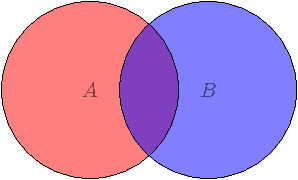
\includegraphics[width=0.25\textwidth]{veto-players-1.pdf}
    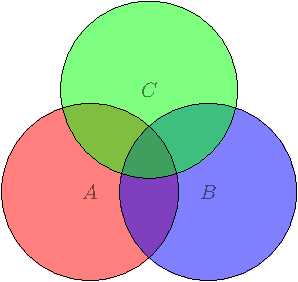
\includegraphics[width=0.25\textwidth]{veto-players-2.pdf}
    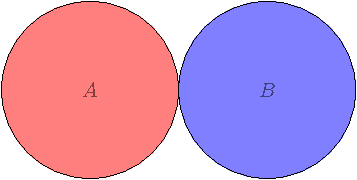
\includegraphics[width=0.25\textwidth]{veto-players-3.pdf}
  \end{center}
  \caption{The overlap between the policies acceptable to veto player
    $A$ and veto player $B$ is shown in the leftmost diagram. In the
    middle, the addition of veto player $C$ has caused the winset to
    become smaller. On the right, the actors $A$ and $B$ have moved
    `ideologically' away from each other, so that there is no winset
    at all outside the status quo.}
\end{figure}

\marginpar{QQ: How much policy stability and government stability
  would there be, if $A$, $B$ and $C$ were veto players in each of
  these diagrams?}

% Block 4.
% From the lecture, and the reading on Environmental Federalism in the
% EU & US by David Vogel
\section{Federalism in the EU and the US}
\begin{flushright}
  \scriptsize Notes from the lecture on the EU and US (Block 4), and
  the reading `Environmental Federalism in the EU \& US' by David
  Vogel (Block 4).
\end{flushright}

\defn{Federation}{Authority is divided between the central state, and
  local governments.}

\defn{Confederation}{Authority is held by independent states and
  delegated to the central governments.}

\defn{Unitary system}{Authority is centrally held with state and local
  governments administering authority that has been delegated by the
  central government.}

\defn{Dual federalism}{National and state governments are split into
  their own spheres, and each is supreme in its respective sphere.}
Based off of the premise that separate but equal branches of
government is the best option.

\defn{New federalism}{Is an idea in the US to transfer certain powers
  ceded by states with Roosevelt's New Deal to the federal government
  back to the states.}

\defn{Cooperative federalism}{Is a concept of federalism in which
  national, state and local governments interact cooperatively and
  collectively to solve common problems, rather than making policies
  separately.}

\subsection{US Federal and State Governments}

The federal government has exclusive powers over war, money, treaties
with foreign countries, regulation of commerce between states, and
powers regarding taxation and welfare.

The state governments have powers to create their own local
governments, conduct elections, regulate commerce within their state,
promote public health, safety, morals, and all other powers that
haven't been delegated to the federal government (this is the 10th
amendment).

Both levels can levy taxes, borrow and spend money, charter
corporations and banks, create and enforce laws, etc.

\subsection{Supranationalism and the EU}

\defn{Supranationalism}{Is the idea that autonomous governing bodies
  have the power and authority to make decisions above the level of
  member states, and in the interest of the supranational body
  (e.g. the EU) as a whole.} As such, we talk about supranationalism
when discussing the EU rather than federalism.

\defn{Intergovernmentalism}{Is the negotiation process among leaders
  of national governments inside a supranational body that leads to
  key supranational decisions.}

\marginpar{QQ: Name an area of governance that the EU has a high,
  shared and supporting competence in.}

The EU has several levels of competence:
\begin{description}
  \item[High/exclusive competence]- Customs union, monetary policy and
    competition law.
  \item[Shared competence] - Environmental policy, consumer protection
    and research.
  \item[Supporting competence] - Civil protection (e.g. police),
    education, culture.
\end{description}

\subsection{Environmental Federalism in the EU and the US}

Environmental regulation in the US has evolved from being state level
to being federal level, and now there is a reciprocity between the
federal government and state governments, where states experiment and
the federal government can learn and encourage conformity. Thus, state
governments are an important source of policy innovation and
diffusion.

\defn{Policy Innovation}{The creation of new and novel policies.}

\defn{Policy Diffusion}{The idea that policies made at a given place
  and time are influenced by policy choices made elsewhere. Horizontal
  diffusion is between governments on the same organizational level,
  and vertical diffusion is (usually) from lower level governments up
  to higher level governments.}

The EU has much closer and important interactions between the
supranational level and the state level because:

\marginpar{QQ: Why is the EU more closely integrated on environmental
  issues (between the EU and individual nations) than the US is?}

\begin{enumerate}
  \item States have direct representation in the EU through the Council
    of Ministers, while in the US, senators and representatives argue on
    behalf of the individual states, but are also have other allegiances
    too (e.g. party politics).
  \item The EU insists on regulatory conformance, but the US does not
    and is happy to diverge. This is partly because the EU's single
    market is new and fragile, so the EU tries to protect it through
    conformity.
  \item Politics moderates where the activities take place. It's not
    politically feasible for federal action on environmental issues to
    take place on the federal level in the US right now, so it happens
    almost exclusively on the state level instead. However, in the EU,
    environmentalism is widespread throughout society, so it happens
    on all levels of the governmental hierarchy.
\end{enumerate}

\section{Communism and Authoritarianism}
\begin{flushright}
  \scriptsize Notes from the lecture in Block 4.
\end{flushright}


There are several forms of authoritarianism, which can be
overlapping:

\defn{Absolute monarchy}{Rulers have absolute power and are defined by
  their hereditary.}

\defn{Totalitarian state}{Authority lies exclusively with the top
  leadership.} North Korea is an example of a totalitarian state.

\defn{Fascist state}{Far right ultranationalist and dictorial
  governments that suppress opposition and strongly regiment society
  and the military.}

\defn{Dictatorship}{Absolute power for the leadership of government.}

\defn{Military Juntas}{The military takes over a country, often to
  `protect democracy'.}

\defn{Communist regimes}{A state that tries to realize the communist
  ideology; to ensure the common ownership of the means of production
  and remove social classes and money.} Communism has an ideological
base, but dictatorships are based purely on power (and the two are not
exclusive.

\marginpar{N.b. Democratic centralism is the idea that party members
  should vote on party matters, and the proletariat doesn't need to be
  political at all.}

Marx and Engels wrote the communist manifesto, and didn't want it to
be a political party. It was originally a class struggle between the
controllers of production (bourgeoisie) and the labour force (the
proletariat).

Lenin made communism political and created the communist party, saying
that democratic centralism is important since the proletariat cannot
be politically aware and the party must be political for them. Lenin's
eventual goal was to create a dictatorship in order to `cleanse' the
proletariat of religion and nationalism.

\marginpar{Agricultural collectivization: Stalin oversaw the creation
  of huge farms, with the idea of automating them with machinery to
  make food plentiful. Peasants were conscripted to work on the farms,
  though they mostly resisted and had no experience of machinery. In
  the end, a lack of equipment, terribly designed farms, monocultures
  and low level peasant resistance meant that food production crashed
  and there was a massive famine in the 1930's.}

\marginpar{QQ: What was the great purge?}

Stalin then took communism to another level, he purged all the people
in the communist party who might not have been fully committed to the
regime (the Great Purge), and installed communist governments in
Central and Eastern Europe (setting the stage for the cold war). He
rapidly industrialized Russia, and enacted collective agriculture.

\marginpar{QQ: Are Perestroika and Glasnost two ideas still embraced
  in Russia today?}

After the cold war, Gorbachev enacted two policies:

\defn{Perestroika}{A shift away from communism towards a market
  economy.}

\defn{Glasnost}{A shift towards open debate.}

\subsection{The Cold War}

The cold war made the world quite stable, because there was a bi-polar
equilibrium, though tension across the world was heightened. Today,
there is more instability but less tension.

\defn{Domino Theory}{Is the idea that when a state becomes communist,
  other nearby states are at risk of becoming communist too.}

\defn{Containment Theory}{Aims to influence capitalist states
  bordering communist states to stop communism from spreading
  according to domino theory.}

Though the cold ware is often thought of being a western oriented
conflict between the US and Russia, lots happened in East Asia
too. China was pitted against Taiwan, and North Korea against South
Korea.

\subsection{China and Communism}

Mao organized China into a one-party communist state. It had (and
still has) a Politburo which is a group of around twenty high ranking
officials that make the big decisions of government.

\marginpar{QQ: What was Mao's strategy of communism in China?}

Mao said that the proletarian revolution that happened in Russia was a
western creation, and focused his ideas on agricultural workers that
were more relevant to China. He tried to break with China's
aristocratic past and planned to make China great through the hard
work of ordinary people. Through this logic, he thought that the more
Chinese people there were, the stronger China would be.

Mao had three big ideological campaigns during his rule, all were
disasters:

\marginpar{QQ: What were the ideological campaigns that Mao ran in
  China during his rule?}

\begin{itemize}
  \item The \textbf{Let One Hundred Flowers Bloom} campaign ('56-'57)
    asked people publicly post ideas for China's future, but then
    killed people who made progressive or good ideas.
  \item \textbf{The Great Leap Forward} ('58-'60) tried to
    collectivize steel production (which failed, producing very low
    quality steel as untrained peasants, who had to actually make the
    steel, had no idea what they were doing, and used any scrap metal
    to fill their quotas). It also tried to kill all the sparrows in
    China since they ate crops, but this just caused a plague of
    locusts which ate more of the crops.
  \item \textbf{Cultural Revolution} ('66-'69, but possibly longer)
    gave power to young people over more established and educated
    people (such as teachers and doctors). Lots of China's cultural
    heritage was destroyed.
\end{itemize}

China was reformed under Deng Xiaoping, who shifted away from
ideological campaigns, shifted away from communism and shifted away
from a socialist economy, to move China slowly towards a market
economy.

\marginpar{QQ: What did Deng Xiaoping do with his reforms?}

Under successive governments, China brought in five-year plans that
focused on economic growth, tried to redistribute wealth from East to
West, tried to fight corruption, and joined international institutions
such as the World Bank.

\marginpar{QQ: What problems does China face now?}

China is now a huge country, with over 1.3 billion people, with a
population growing at 4.2\% and a GDP growing at 9.3\%. However, China
is very multi-ethnic, and has lots of income inequality, an
undercurrent of political unrest, severe pollution and resource
depletion. It must face those challenges in the years to come.

% Block 5
% Taken from 'Policy Diffusion: Seven Lessons for Scholars and
% Practicitioners' by Shipan and Volden.
\section{Policy Diffusion - Seven Key Points}
\begin{flushright}
  \scriptsize Notes from 'Policy Diffusion: Seven Lessons for Scholars
  and Practitioners' by Shipan and Volden (Block 5).
\end{flushright}

\marginpar{QQ: Give as many key points about policy diffusion as you
  can.}

Policies do not exist in isolation; governments learn from each other,
calibrate their policies against one another, and policy advocates
target their efforts accordingly.

\begin{enumerate}
  \item \textbf{Policy Diffusion is not limited by geographic
      constraints}. Governments look all over the world for successful
    policies to co-opt into their own programmes, and are rarely
    limited by geography; why should they be?
  \item \textbf{Governments compete with each other} to attract or
    repel residents or business. For example, if middle-class
    families are flocking to an area with good schools, other areas
    might try to improve their schooling policies to attract them
    back, or they could try to improve policies in other areas for the
    same effect. Conversely, a race-to-the-bottom can also happen in
    order to repel people away from somewhere, for example, if welfare
    is very good in one city, then it could attract many people in
    need and put a large burden on the city.

    Sometimes, governments don't need to compete (for example, on
    youth access to tobacco), or agree not to compete, or even to act
    together (for example, through trade agreements).
  \item \textbf{Governments learn from each other}. Individual
    governments can experiment, and other governments can take the
    successful ideas. That said, policy makers could have a wide
    variety of objectives when learning from other governments, and
    they might not always be in the public good. For example, some
    policy makers could try to pick policies that get politicians
    reelected.

    Low cost communication and travel means that it's easier than ever
    for policy makers to exchange information, and many networks of
    policy makers exist to facilitate this.
  \item \textbf{Policy diffusion isn't always beneficial}. As
    previously noted, competition can produce a race to the bottom
    among states, but there are two other negative occurrences.

    \defn{Policy Imitation}{Is when one government copies another's
      successful policies without assessing whether the context in
      which the policies were successful applies to their own
      government's situation.} This means the policies are often
    inappropriate.

    \defn{Policy Coercion}{Is when force (either hard or soft) is
      applied by one government to another to make it adopt a certain
      policy. The US does top-down policy coercion when it attaches
      conditional restrictions to development grants, and the IMF does
      it when it pushes austerity policies on struggling governments.}
  \item \textbf{Government capabilities are important}. Many
    governments adopting a policy could have a `snowball' effect,
    causing it to be more likely to be adopted everywhere. However, if
    many subordinate (e.g. local) governments adopt a policy, then it
    could also act as a `pressure valve' and take pressure off the
    higher-level (e.g. state) government to act.

    Some governments have a low capacity, for example they may not pay
    legislators enough, or have very few staff. These governments are
    likely to exhibit the pressure valve effect since it's less work,
    or just not look elsewhere for suitable policies, or blindly adopt
    policies.
  \item \textbf{Some policies spread more easily than others}. Complex
    policies spread more slowly than simple policies. Likewise,
    policies that have observable effects, confer a relative advantage
    on the legislating government, and are easily testable are more
    likely to be diffused.
  \marginpar{QQ: Why is decentralized governance important for policy
    diffusion?}
  \item \textbf{Decentralization is important for policy diffusion},
    since experimentation is critical for the creation of new and
    novel policies that other governments can copy. If centralization
    occurs, then horizontal diffusion is stifled, and local
    governments cannot match policies to local
    preferences. Higher-level governments can mitigate this by
    mandating local policy experimentation, for example, local
    governments could be required to come up with an interpretation of
    a policy, thereby artificially creating policy experimentation.
\end{enumerate}

% Block 5
% Based on the lecture slides & my lecture notes.
% Unfortuately, the below is all I had, so I'm leaving this out.
%\section{Political Parties}

%\textit{Note that at the time of writing, the lecture notes are in
%  German, any my own German skills combined with Google Translate
%  don't do a great job of making it understandable. As such, these
%  notes are made up from my own notes from the lecture.}

%Political parties are organizations of people with similar ideas that
%are formed in order to win elections and control government.

%They originated with the Whig party (who against an aboslute monarchy
%in the UK) and the Tory party (who were for it).

%The role of political parties is to nominate candidates for elections,
%help pick the best person to run, actually govern after they are
%elected, and act as a watchdog in the political process.

% Block 6
% Based off the lecture notes, with a little input from the reading
% "Streams and Stages; reconciling Kingdon and Political Process
% Theory" (which I found hard to really get much out of)
\section{Multiple Streams and Policy Windows}
\begin{flushright}
  \scriptsize Notes from the lecture, with a little input from the
  reading ``Streams and Stages; reconciling Kingdon and Political
  Process Theory''. Block 6.
\end{flushright}

\defn{Policy}{A principle, plan, or course of action, as pursued by a
  government, organization, individual, etc.}

\defn{Policy Making}{The act or process of setting and directing the
  course of action to be pursued by a government, business, etc.} It
can occur on many levels.

There are multiple kinds of decision making:
\begin{description}
  \item[Organizational decision making] selects the best solution for an
    identified problem.
  \item[Incremental, routine decisions] are decisions that happen
    repeatedly (this is the most common)
  \item[Incremental, non-routine decisions] are the subject of this
    section.
\end{description}

\subsection{Rational Decision Making}

\marginpar{QQ: What is the pattern of rational decision making?}

Rational decision making follows a pattern of problem identification,
solution identification and evaluation and the deciding on a solution
and implementing it. It assumes full information, decision makers
powerful enough to carry out a decision, and agreement on the best
course of action.

Key concepts include:

\defn{Satisficing}{Limiting the range of information examined in
  identifying problems and solutions because information gathering is
  expensive.} For example, one could assume that Coronavirus behaves
in the same way as SARS did, because there's no opportunity to test it
further.

\defn{Bounded rationality}{Decision making and rationality of
  individuals is limited by the information they posses, the cognitive
  limitations of their minds, and the finite time they have to make a
  decision.}

\defn{Negotiated decisions}{Compromise, bargaining, accommodation among
  parties/interests/coalitions in making a decision (decision making
  is affected by values and preferences of decision makers).}

\subsection{Incremental Decision Making}

\marginpar{QQ: Who said what about incremental decision making?}

Decision makers often make choices similar to those made in the
past. Charles Lindblom describes it as ``the science of muddling
through''. An incremental decision making mindset doesn't consider the
entire range of possible information about possible solutions, but
instead considers only information relevant to extending the current
policy.

\subsection{The Garbage Can Decision Making Model}

\marginpar{QQ: Who proposed the garbage can model?}

Proposed by Cohen, Marsh and Olsen in 1972, the Garbage Can model
imagines that there is a garbage can full of solutions to problems,
and when a problem arises, policy makers randomly pick a solution from
the can and try to apply it. The decision making process is chaotic,
and bound by many constraints (lots of actors, limited time, etc).

\subsection{Kingdon's Multiple Streams}

\marginpar{QQ: Which stages of the policy making process does Kingdon
  focus on?}

\defn{Agenda Setting}{Is setting the process that determines which
  issues officials pay serious attention to at any given time.}
Kingdon asked why some problems come to occupy the attention of
government officials more than others? Note that Kingdon is concerned
with the agenda setting stage of the policy making process, not later
stages such as the implementation or evaluation stages. That is to say
that if the Policy Cycle is as follows, Kingdon is concerned with
parts one, two and three:

\marginpar{QQ: List the five stages of the policy cycle.}

\begin{enumerate}
  \item Problem recognition
  \item Agenda setting
  \item Policy formation
  \item Decision
  \item Implementation
  \item Evaluation (and possible back to the start if changes are required)
\end{enumerate}

\marginpar{QQ: List Kingdon's three streams, what are they?}

Kingdon proposed five interacting elements:
\begin{enumerate}
  \item The Problem Stream (things like coronavirus, a housing bubble,
    road maintenance, etc). Policy makers must be persuaded to pay
    attention to a particular problem (called agenda setting). This
    involves the framing of events, and focusing attention on them.
  \item The Policy Stream (solutions looking for problems). Policy
    proposals are generated, debated, revised and proposed
    here. Policies that are implementable, align with political values
    and are low-cost are often preferred.
  \item The Politics Stream (parties fighting for attention). This
    includes all the political factors that influence the agenda
    (everything that could open a policy window), including changes in
    elected officials, the political mood, and what advocacy groups
    are focusing on.
  \item Policy Windows (moments with decision making potential).
  \item Policy Entrepreneurs (who focus attention on a problem in the
    middle of everything). These people are elected officials, career
    civil servants, lobbyists, academics, etc. They try to highlight
    indicators of the problem, push for a particular definition of the
    problem, present specific policies (from the policy stream) that
    are solutions to problems (from the problem stream) on the agenda
    (defined by the politics stream), and try to shape the
    debate. Policy entrepreneurs attempt to shape how see a problem in
    order to put forward the solutions they prefer.
\end{enumerate}

\marginpar{QQ: Give examples of policy windows opening.}

In Kingdon's model, the three streams are largely distinct from each
other, but if they all align, then a policy window occurs. Typically,
policy windows don't open for vary long. They can open predictably
(such when an election happens) not always (such as due to a financial
crash). For example, in the financial crisis (a problem from the
problem stream), austerity (a solution from the policy stream) was
pushed by economically conservative figures (policy entrepreneurs).


% These notes are taken from Stephen Luke's "Faces of Power".
% I only read the introduction, but it seems pretty good (if
% intense) so I might read more...
% This is in Block 6.
\section{Faces of Power}
\begin{flushright}
  \scriptsize Notes from Stephen Luke's ``Faces of Power''. I only
  read the introduction, but it seems pretty good, so maybe I'll read
  more... Block 6.
\end{flushright}

Lukes describes two political scientists; \textit{Mills} and
\textit{Hunter}, who in the 50's, described how power was concentrated
in the hands of a small elite, at least inside American society. These
were the people running big corporations, the military, etc, those who
``occupy a strategic command post of the social structure''. They act
as power brokers, mediated through luncheon clubs and fraternities.

Dahl, writing at the end of the 50's disagreed with these theories on
the grounds that they didn't have any empirical backing. In order to
gain scientific rigor, the hypothesis would need to be tested and
meet the following criteria:

\begin{enumerate}
  \item The hypothetical ruling elite is a well defined group.
  \item There is a fair sample of cases involving key political
    decisions, in which the preferences of the hypothetical ruling
    elite run counter to those of any other likely group that maybe
    suggested.
  \item In such cases, the preferences of the elite regularly prevail.
\end{enumerate}
  
In his studies, Dahl found that different actors and different
interest groups prevailed in different issue-areas, with no overall
`ruling elite', meaning that power was distributed \textit{plurally}.

The question the morphed, into one of how `power' should be
defined. Three `faces' that are described are as follows:

\marginpar{QQ: What are the three faces of power?}

\begin{description}
  \item[The first face] is the power of concrete decisions.
  \item[The second face] is the power to limit decision making by
    influencing community values and political procedures.

    Specifically, all organizations have `bias' towards some
    conflicts and away from others. This bias can suppress some
    conflicts so that the status quo is more easily accepted.

    According to Gramsci, this culture/ideology is facilitated by the
    consent or acceptance of normal people, which was voluntary and
    can vary in intensity. If the culture is hegemonic, then the
    conflicts/issues suppressed by the cultural bias are systemic.

    There's lots more on this, ``Faces of Power'', it's interesting.
  \item[The third face] is the power to prevent people, to whatever
    degree, from having grievances by shaping their perceptions,
    cognitions and preferences in such a way that they accept their
    role in the existing order of things.

    In other words, the third face enables power to work against
    people's interests and mislead them so that their judgment is
    distorted.
\end{description}


